\section{Validation with Data from PDS Prototypes}
\label{sec:dp-pds-prototypes}

The \dword{lar} \dword{tpc} \dword{dp} proposed technology is the result of years of R\&D. From small-scale chambers to the \dword{dune} module, many prototypes have been constructed, each with some design modifications and optimizations. 
Relevant to the \dword{pds} itself, the \dword{wa105}, operated at CERN in 2017, the \dword{pddp}, to be commissioned in 2019 and the \dword{dune} far detector module similarities and differences will be described here.

\subsection{Design Similarities and Differences Between Prototypes and FD System}

The first metric ton scale \dword{dp} \dword{lartpc} demonstrator took cosmic data between June and November \num{2017} at CERN. 
Located \SI{1}{m} below the charge collection plane, underneath the cathode and the \dword{gg}, the photon detection system consisted of five \dwords{pmt} (Hamamatsu R5912-MOD20, described in more detail in Section~\ref{sec:dp-pds-photosensors}) evenly distributed along the 3$\times$1~m$^2$ area (one \dword{pmt} every \SI{50}{cm}). The demonstrator was an opportunity to test different \dword{pds} designs, particularly the \dword{tpb} coating and \dword{pmt} bases. Three \dwords{pmt} had the \dword{tpb} coating applied directly onto their windows using evaporation, but for the other two, the \dword{tpb} was deposited on a \SI{4}{\mm} thick transparent Plexiglass plate mounted on top of the \dwords{pmt}. 
While the latter solution has the advantage of being simpler and less risky to manipulate, it reduces acceptance and possibly efficiency because of the internal reflections between the \dword{tpb} and the Plexiglass surfaces. 
Pictures of the \dword{wa105} \dword{pds} are shown in Figure~\ref{fig:pd-pds-311-pmt-tpb}.

\begin{dunefigure}[WA105 PDS ]{fig:pd-pds-311-pmt-tpb}{The \dword{wa105} \dword{pds}. Top left: \dword{pmt} with the \dword{tpb} deposited on the plexiglass plate; top right: \dword{pmt} with the \dword{tpb} coated onto the photocathode; bottom: The five \dwords{pmt} installed in the \dword{wa105} underneath the ground grid.}
%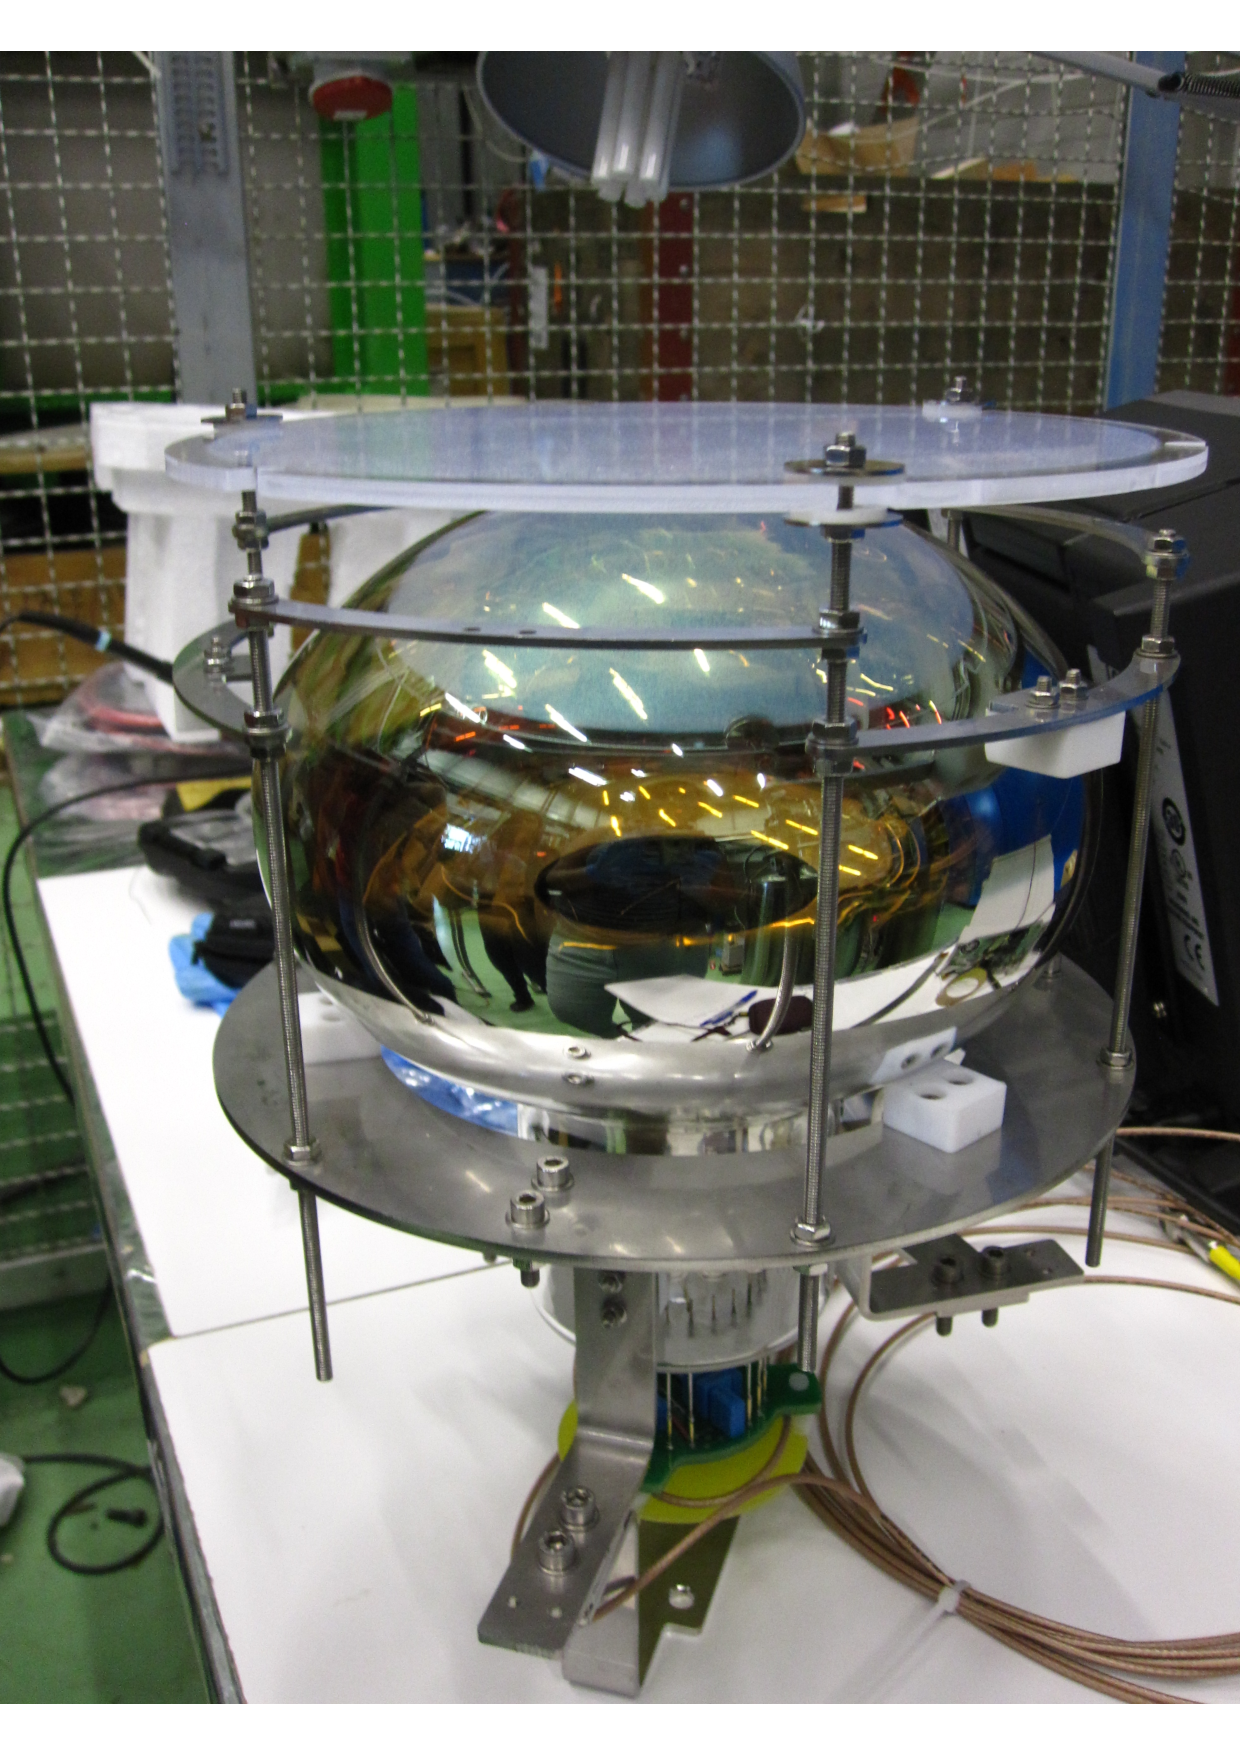
\includegraphics[width=0.25\textwidth]{graphics/dppd_PMTPlate}
%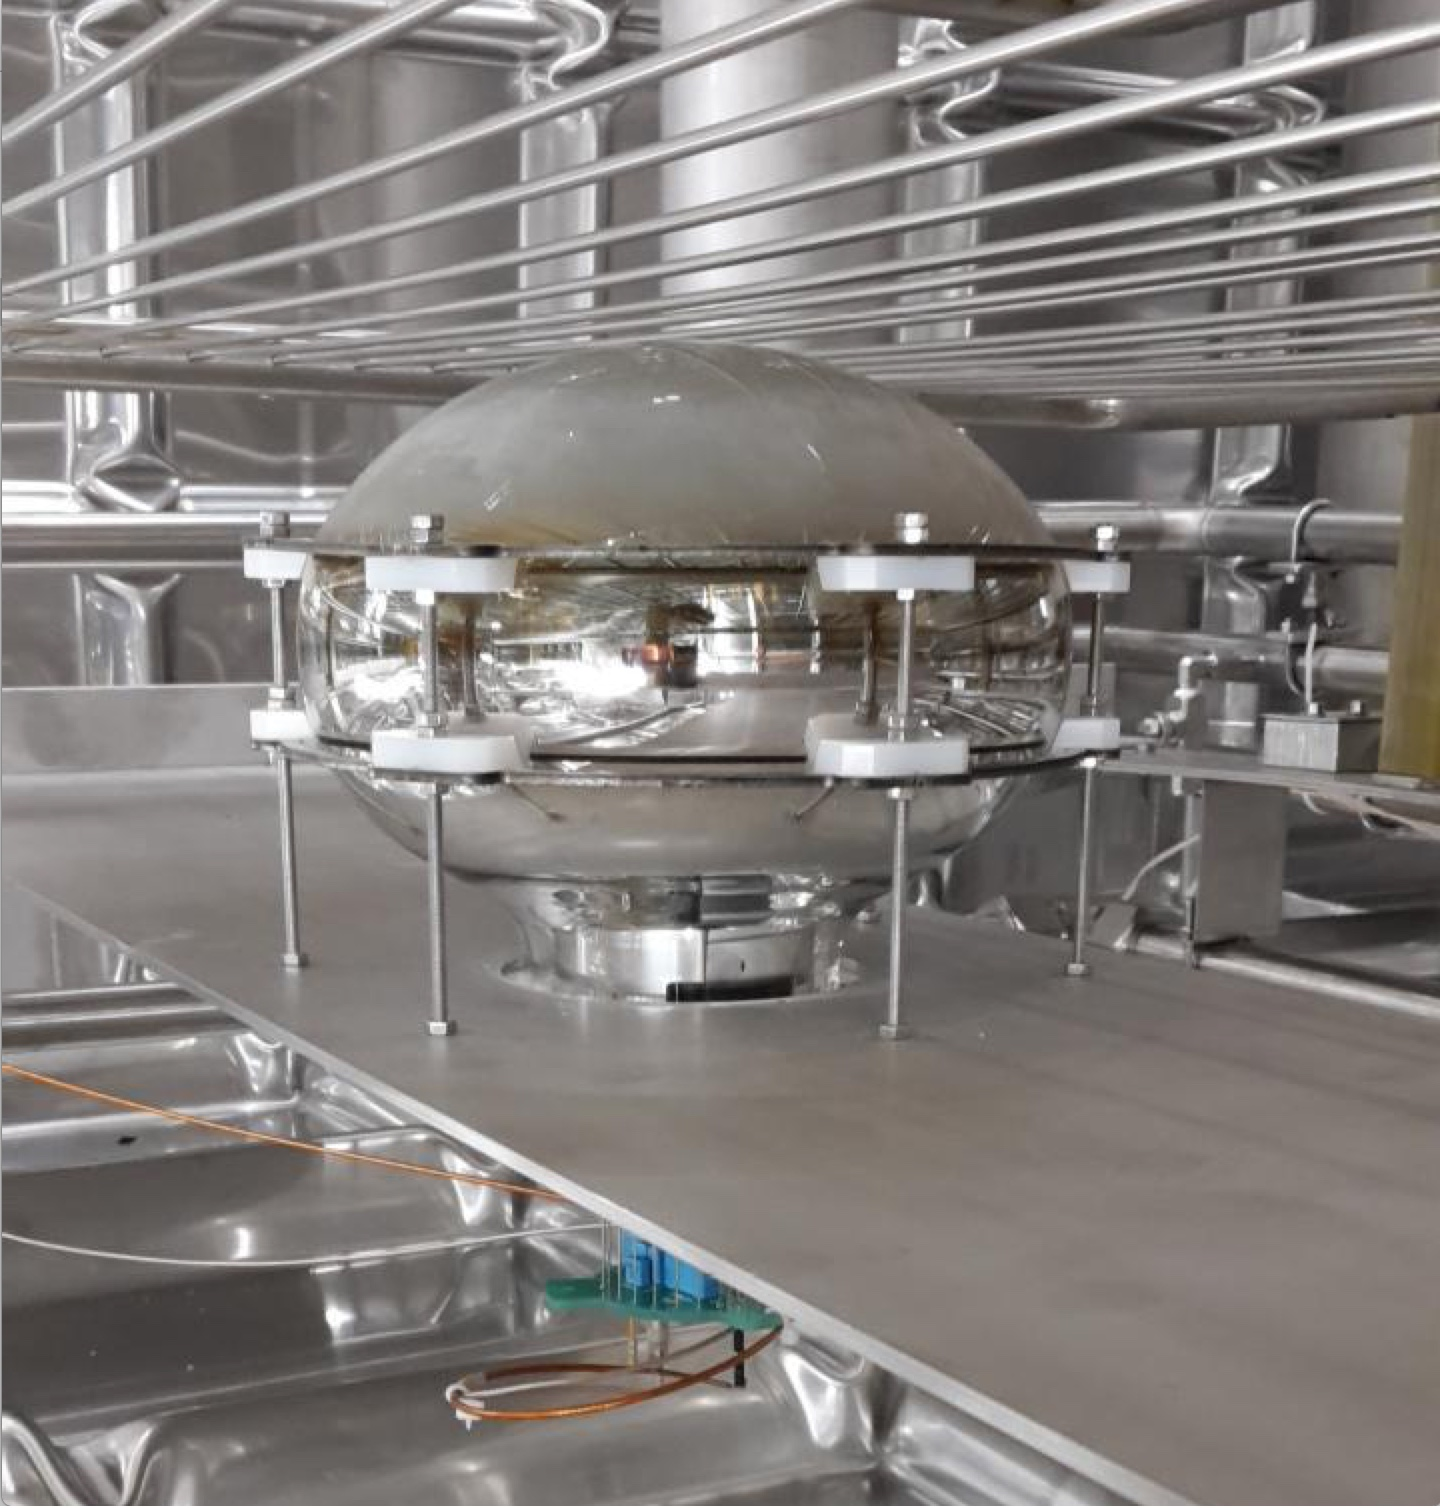
\includegraphics[width=0.33\textwidth]{graphics/dppd_PMTTPB.jpeg}\\
%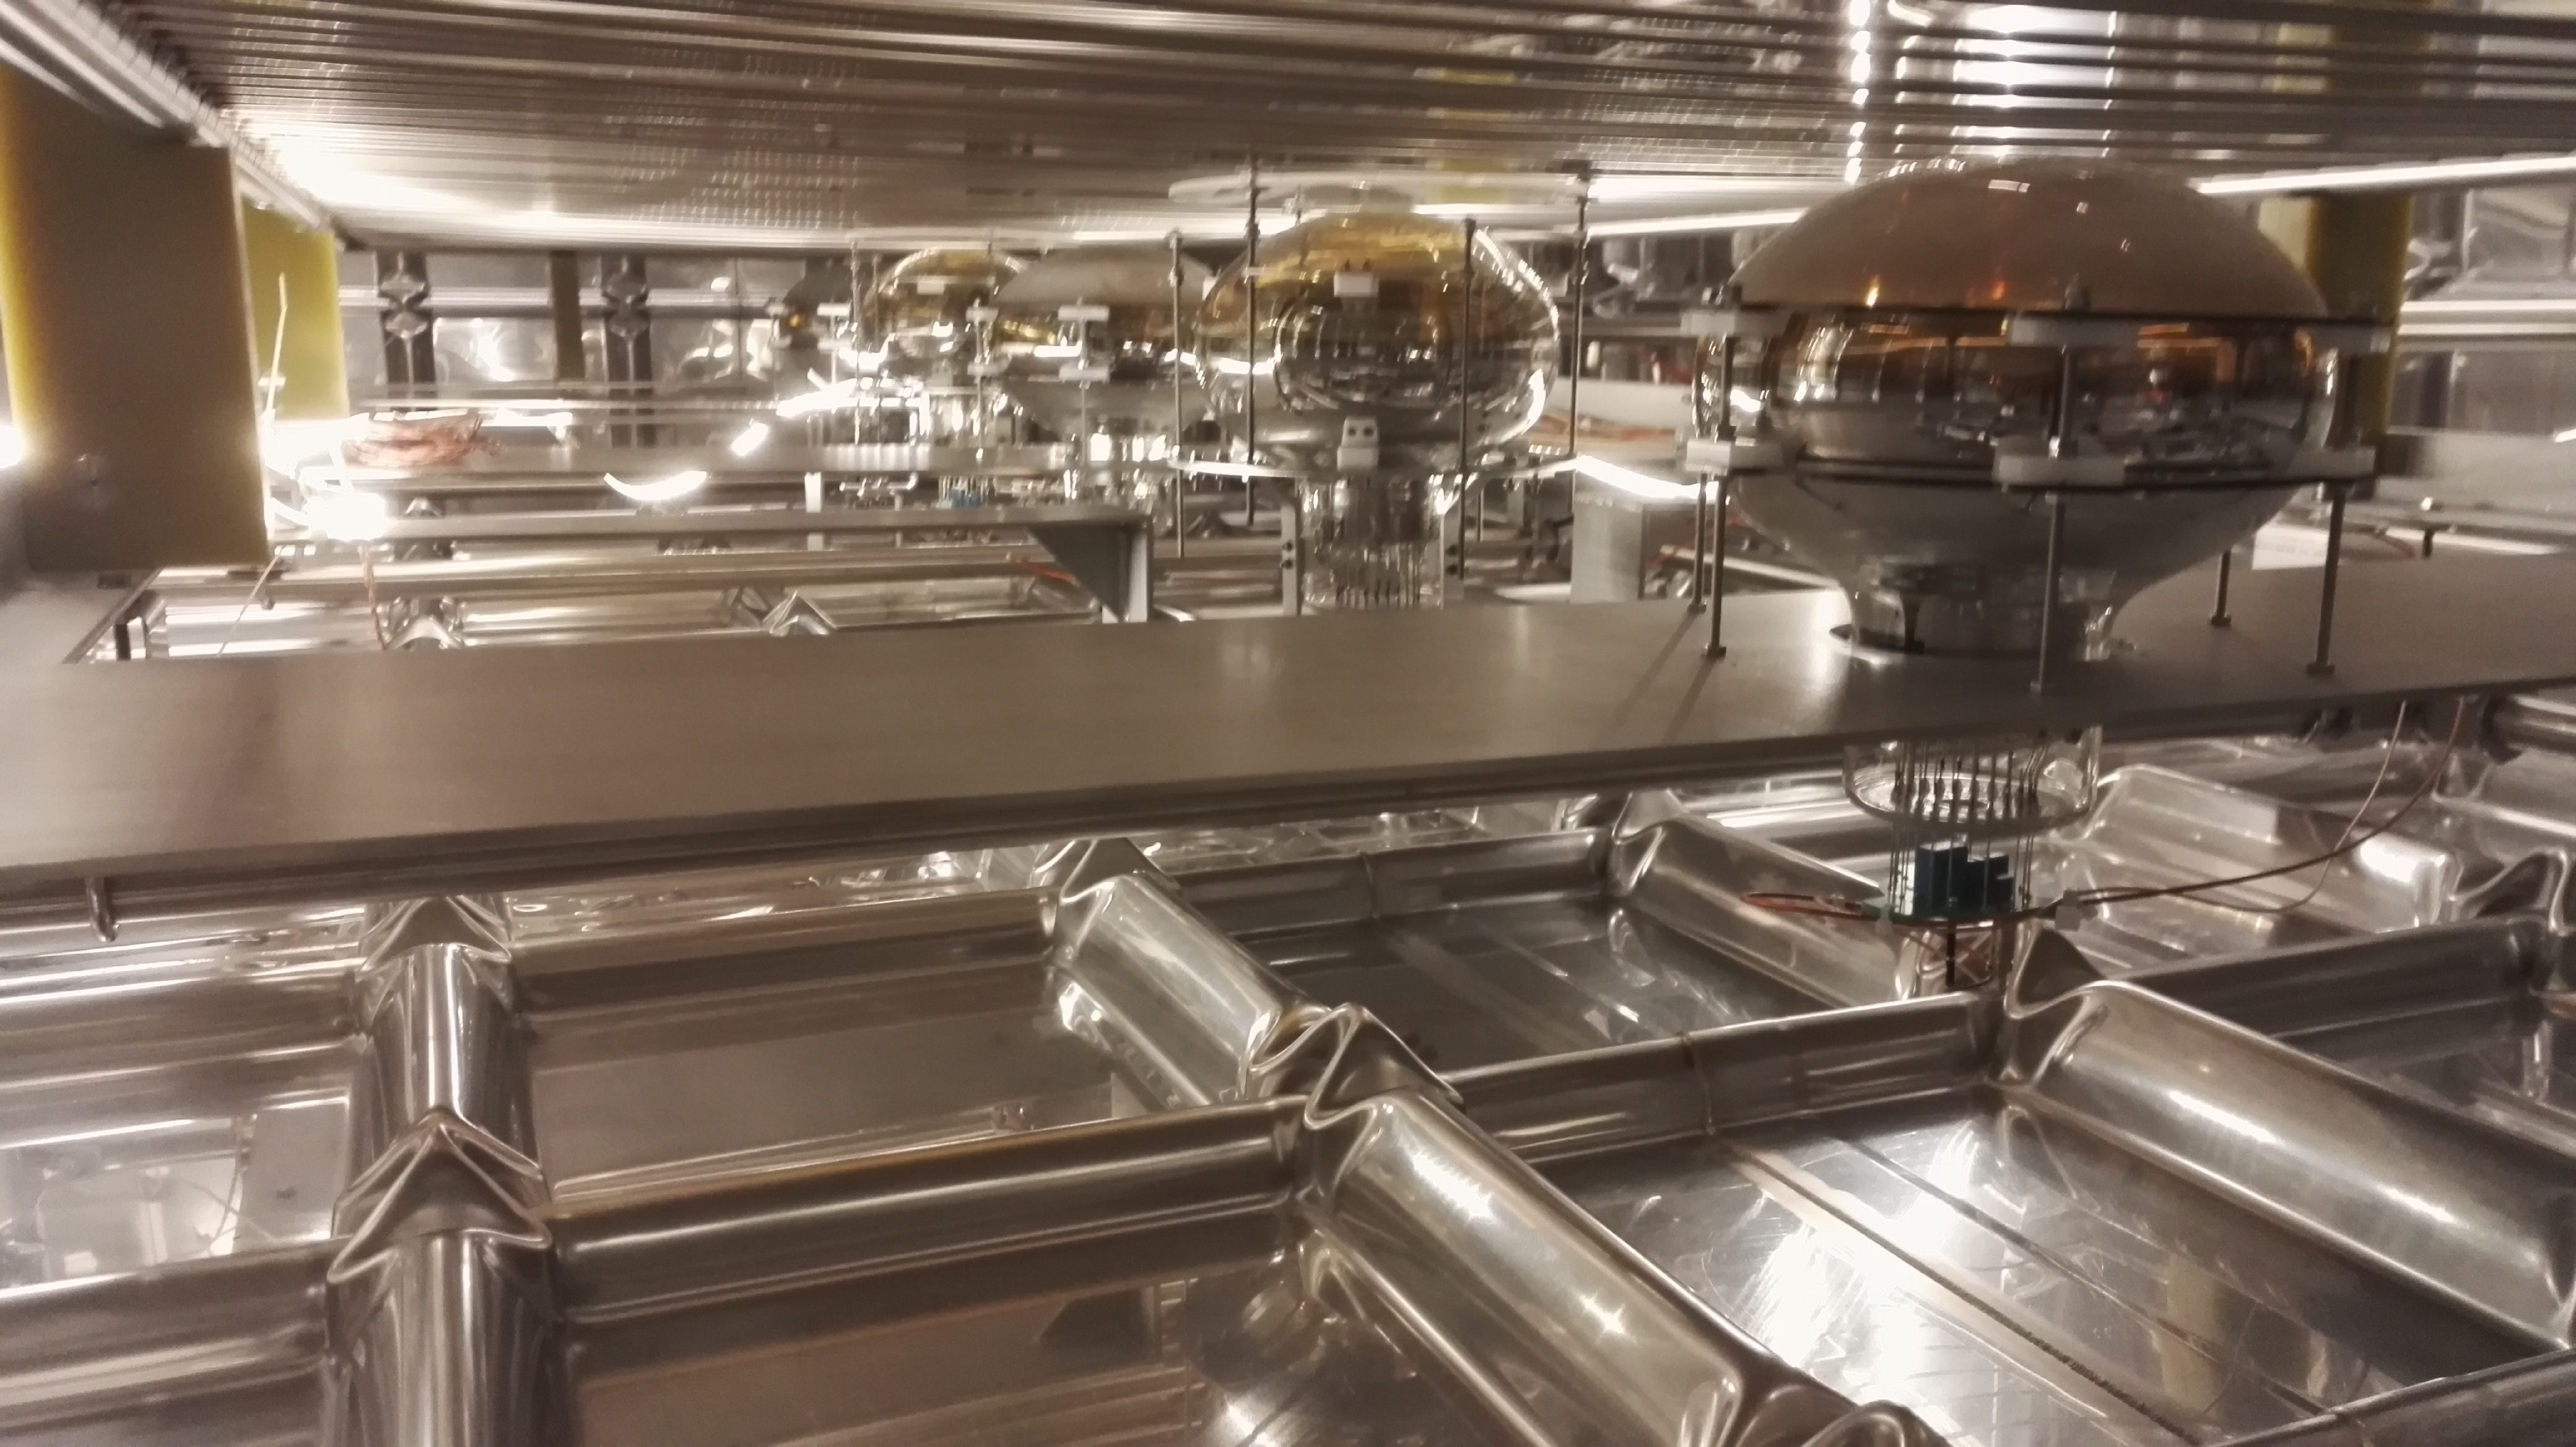
\includegraphics[width=0.6\textwidth]{graphics/dppd_PMT_311_installation.jpg}
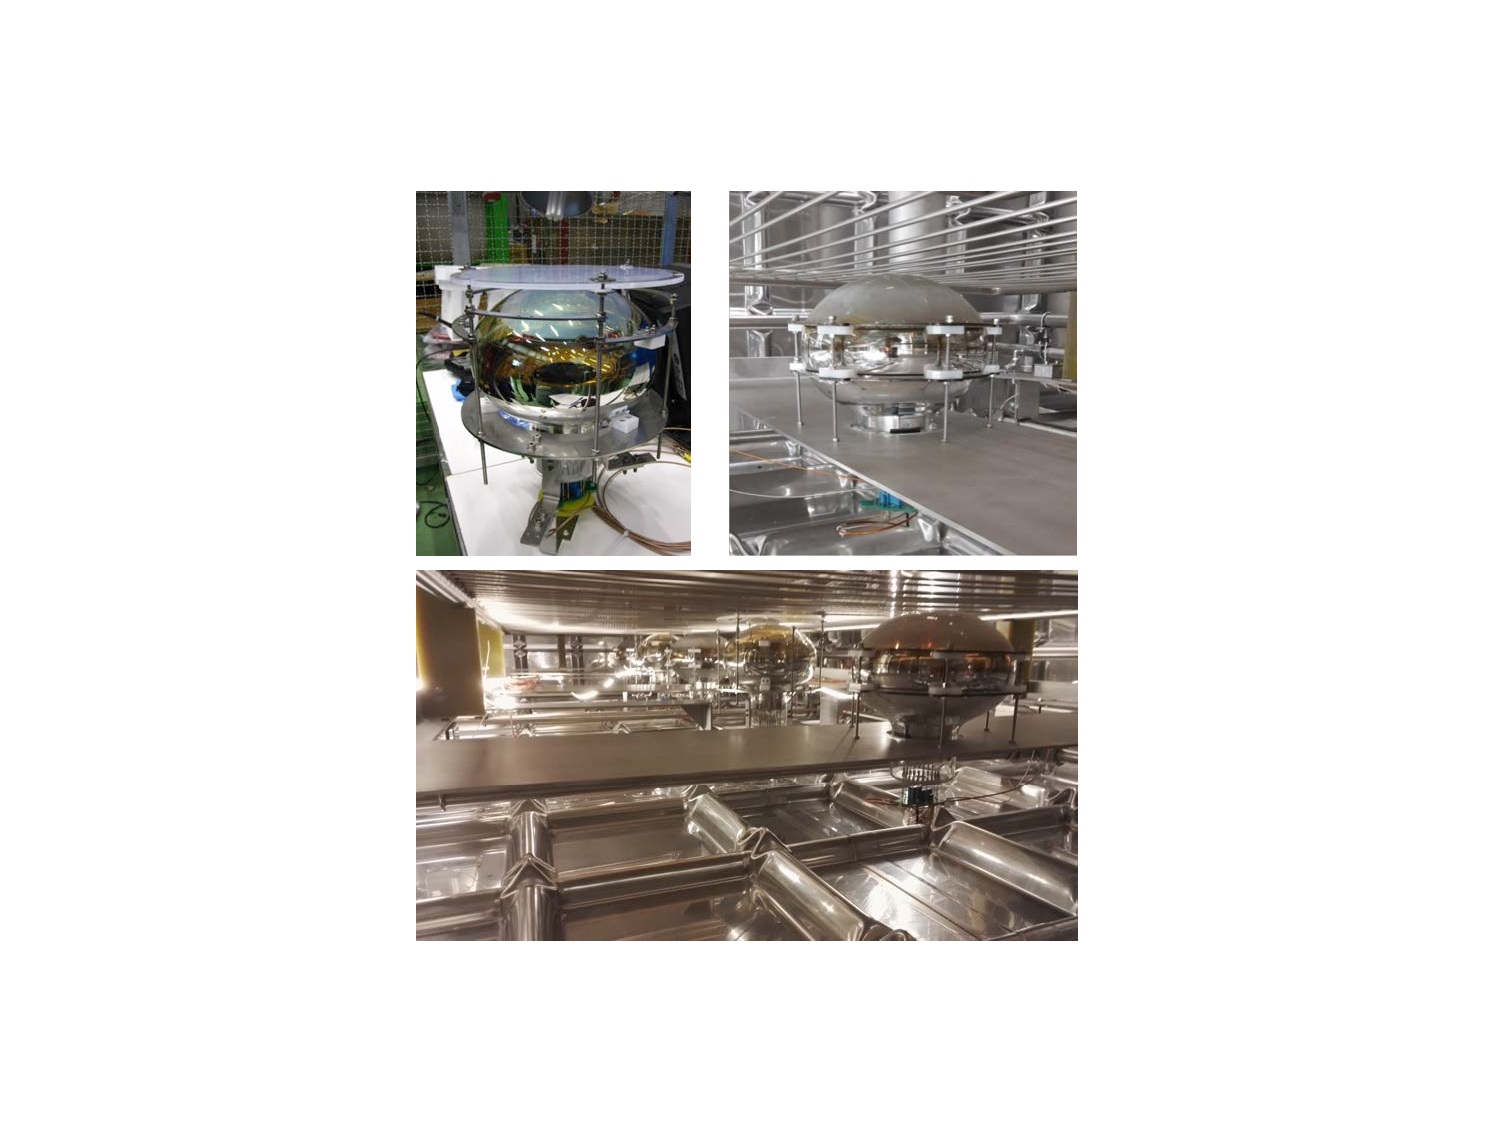
\includegraphics[width=0.5\textwidth]{dppd_311_PMT_combined}
\end{dunefigure}

Two power supply polarities were used. Three \dwords{pmt} were equipped with a negative \dword{hv} base, i.e. a negative bias voltage was applied to the photocathode, and the anode was grounded. This system requires two cables: one for the \dword{hv} system and one for the signal. A positive base served the other two \dwords{pmt}: a single cable positively biased the anode and carried the signal, and the cathode was grounded. The \dword{hv} and the signal were then externally decoupled using a splitter, see Section~\ref{sec:fddp-pd-4.2}. The latter design has the advantage of reducing the number of feedthroughs and cables while also reducing the noise. Overall, four configurations were tested (see Table~\ref{tab:dp-pds-311conf}). During the 3$\times$1$\times$1~m$^3$ operation, the \dwords{pmt} operated at a rather uniform gain of around \num{e6} with a readout sampling of \SI{250}{MHz}.

\begin{dunetable}
[WA105 PMT configurations]
{cccccc}
{tab:dp-pds-311conf}
{Configuration of the five \dwords{pmt} installed in the \dword{wa105}.}
\dword{pmt} & Base & Coating & Voltage (kV) & Gain (\num{e6}) & Noise (ADC)\\ \toprowrule
%\hline
1 & Negative & Coating & \num{-1.2} & 0.92$\pm$0.13 & \num{0.7} \\ \colhline
2 & Negative & Plate   & \num{-1.2} & 1.01$\pm$0.12 & \num{0.7} \\ \colhline
3 & Positive & Coating & \num{1.1} & 0.95$\pm$0.11 & \num{0.4} \\ \colhline
4 & Positive & Plate   & \num{1.1} & 1.26$\pm$0.15 & \num{0.4} \\ \colhline
5 & Negative & Coating & \num{-1.2} & 1.33$\pm$0.15 & \num{0.8} \\
%\hline
\end{dunetable}

In \dword{pddp}, \num{36} \dwords{pmt} are installed \SI{6}{\m} below the collection plane, again underneath the cathode and the \dword{gg}. The \dword{pmt} density is lower than the demonstrator. Their positioning over the \SI{36}{m$^2$} area was optimized with simulations. The number of \dwords{pmt} is higher around the center of the active volume and lower near the \dword{fc} borders. This positioning maximizes the amount of light collected from cosmic rays.

After evaluating the demonstrator configurations, the \dword{tpb} was directly evaporated onto the \dword{pmt} windows, and the \dword{pmt} base was chosen to have positive polarity. This configuration maximizes collection efficiency and reduces both the number of cables and the electronic noise. 

For \dword{dune} \dword{fd} \dword{pds}, \dword{tpb} will be directly applied to the \dword{pmt} windows, and the positive biasing scheme will be implemented. The aspect ratio between cathode size and drift distance is larger than in \dword{pddp}, so the amount of light loss by absorption on the \dword{fc} should be smaller. Therefore, the \dword{dune} \dword{fd} \dword{pds} layout should be uniform with \dwords{pmt} on a regular lattice with \SI{1.02}{m} spacing. On the other hand, light attenuation due to absorption in the \lar itself will be larger in the \dune \dpmod.

%%%%%%%%%%%%%%%%%%%%%%%%%%%%%%%%%%%%%%%%%%%%%%%%%%%%%%%%%%%%%%%%%%%%

\subsection{\dword{wa105} Light Data Results and Simulation Validation}

Analysis of data taken during the \dword{wa105} operation provides the first validation of and improvements in the light simulation developed so far. 
The demonstrator ($3\times1\times1$~m$^3$ active volume) has linear dimensions comparable with the Rayleigh scattering length, which is approximately \SI{60}{\cm}. 
As a consequence, the light absorbed by elements of the detector (such as the \dword{fc}, \dword{lem}, or cathode) may become a problem.
Hence, light maps were created with particular care for precision in reproducing the demonstrator's geometry.

Two triggering schemes were used during the \dword{wa105} operation.
The first was provided by an external muon tagger, the \dword{crt}, to record horizontal muons. The \dword{crt} was made of plastic scintillator planes on each side of the detector.
The second was provided by the \dwords{pmt} themselves, requiring that the five sensors record sufficient light in coincidence. In this configuration, more vertical muons and showers were recorded.

Using the \dword{crt} trigger condition, a rough track reconstruction is possible because the \dword{crt} provides coordinate information with \SI{11}{\cm$^2$} resolution. Hence, even without charge information, as for data taken at null field, it is possible to select muon-like tracks and retrieve the shortest distance between the track and each \dword{pmt}. A schematic drawing of the \dword{wa105} detector is presented in Figure~\ref{fig:pd-pds-311schema} with the relevant track parameters.

\begin{dunefigure}[WA105 schematic drawing]{fig:pd-pds-311schema}{Schematic view of the \dword{wa105}. 
The fiducial volume is in gray and limited from the collection plane area to the cathode. The active volume is in yellow. Its volume is defined by the collection plane: the \dword{fc} to the top of the \dwords{pmt}. A track that would be detected by the \dword{crt} is shown with its minimum distance to \dword{pmt} \num{3} in red.}
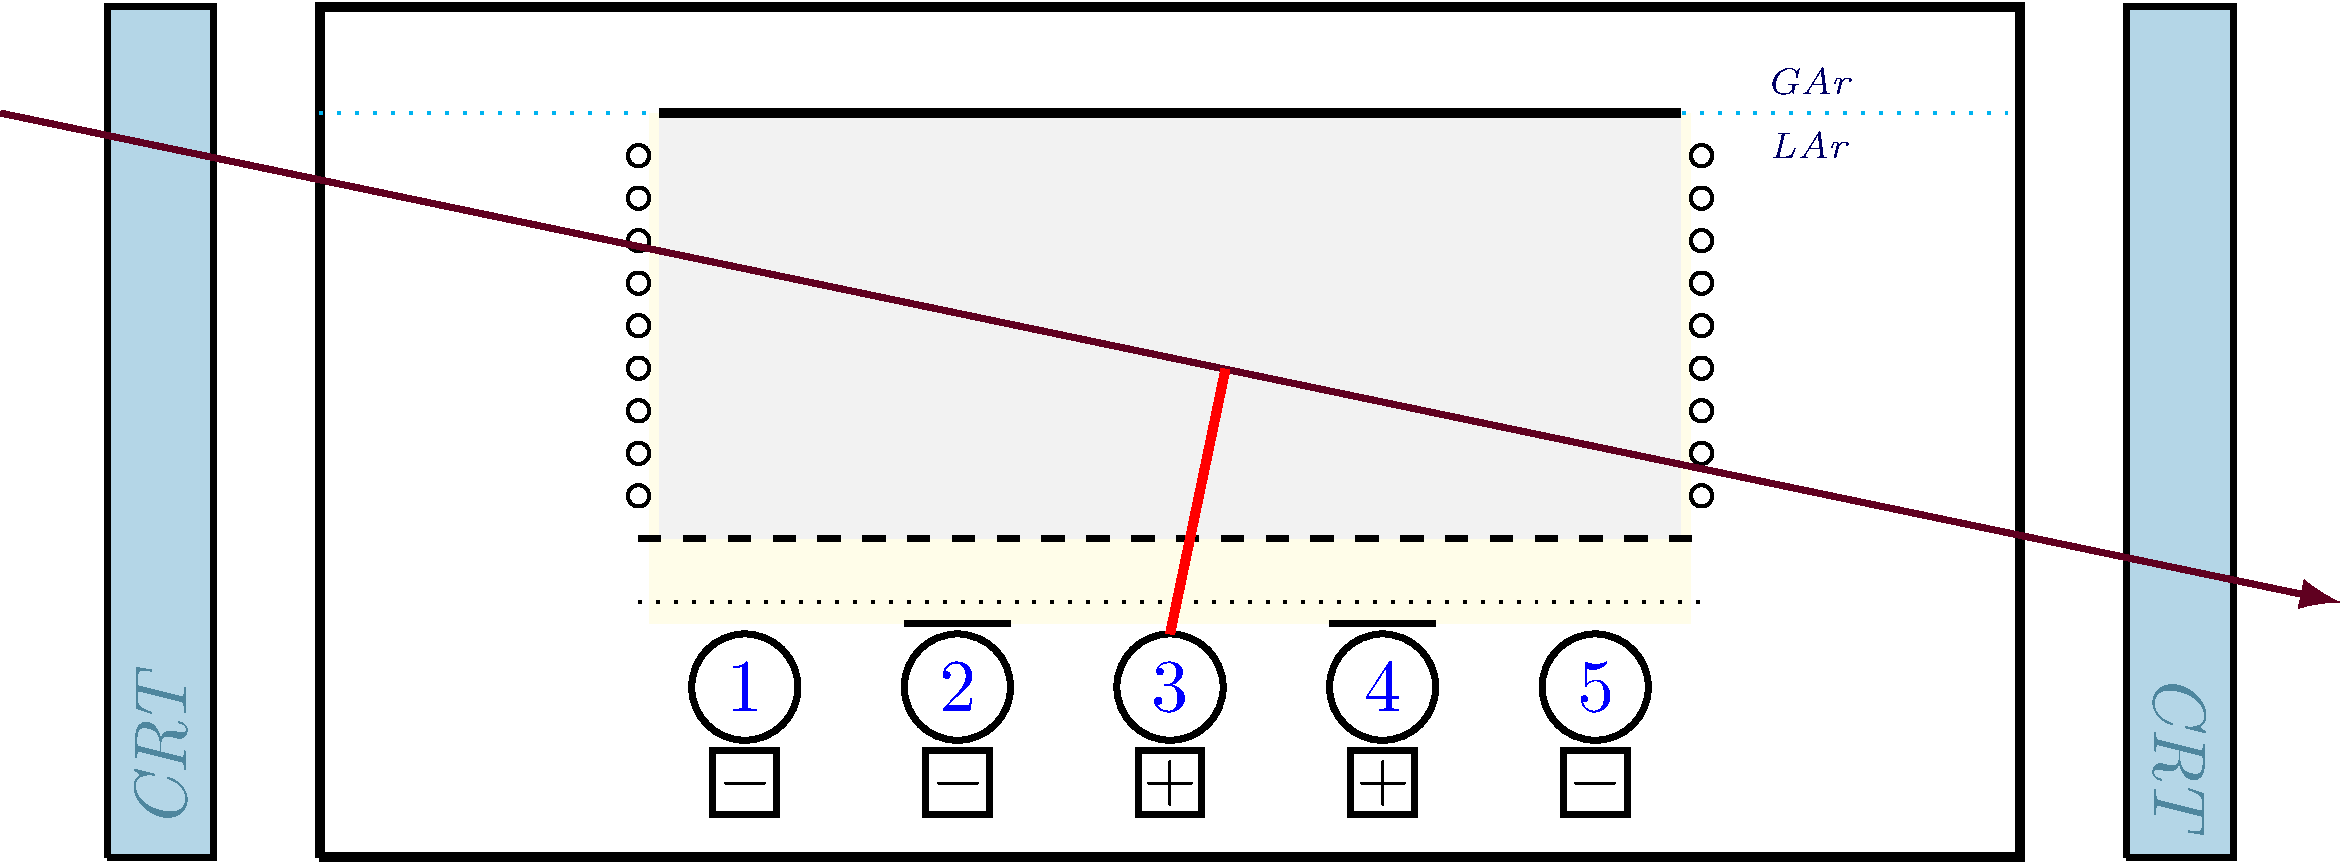
\includegraphics[width=0.75\textwidth]{graphics/dppd_7_2_v2}
\end{dunefigure}

From the \dword{pds} point of view, the \dword{wa105} operation lasted several months because light was collected during cool down, filling, and commissioning stages of the demonstrator.
The \dword{pds} performed with high stability during this entire period. 
In Figure~\ref{fig:pd-pds-311-ped}, the  pedestal mean and \dword{rms} are shown for one positive and one negative base \dword{pmt} as a function of time for \num{5} months of operation. 

\begin{dunefigure}[WA105 PMTs mean pedestal and RMS]{fig:pd-pds-311-ped}{Pedestal mean (top) and \dword{rms} (bottom) for one negative base \dword{pmt} (black) and one positive base \dword{pmt} (red) between July and December 2017 during the operation of the \dword{wa105}.}
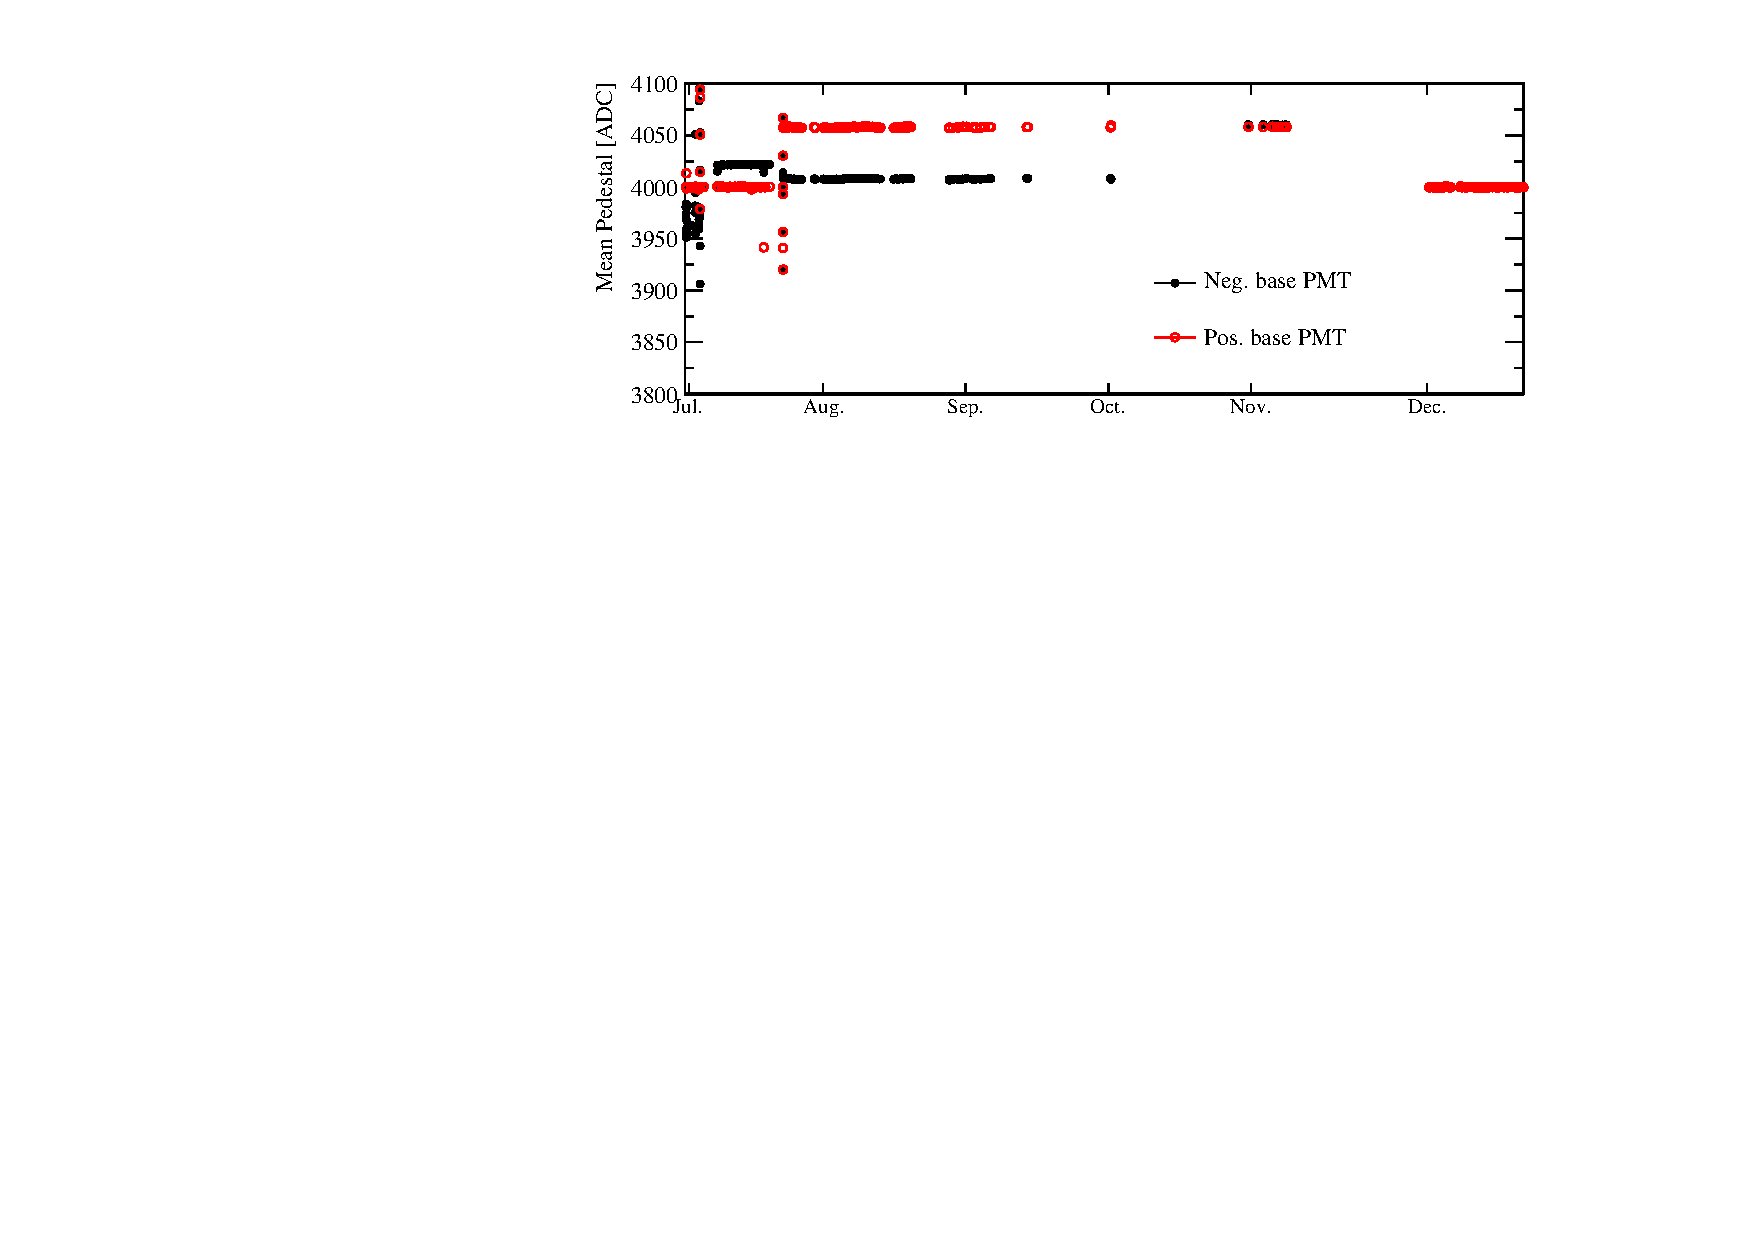
\includegraphics[width=0.9\textwidth]{graphics/dppd_311_pedestal.pdf}\\
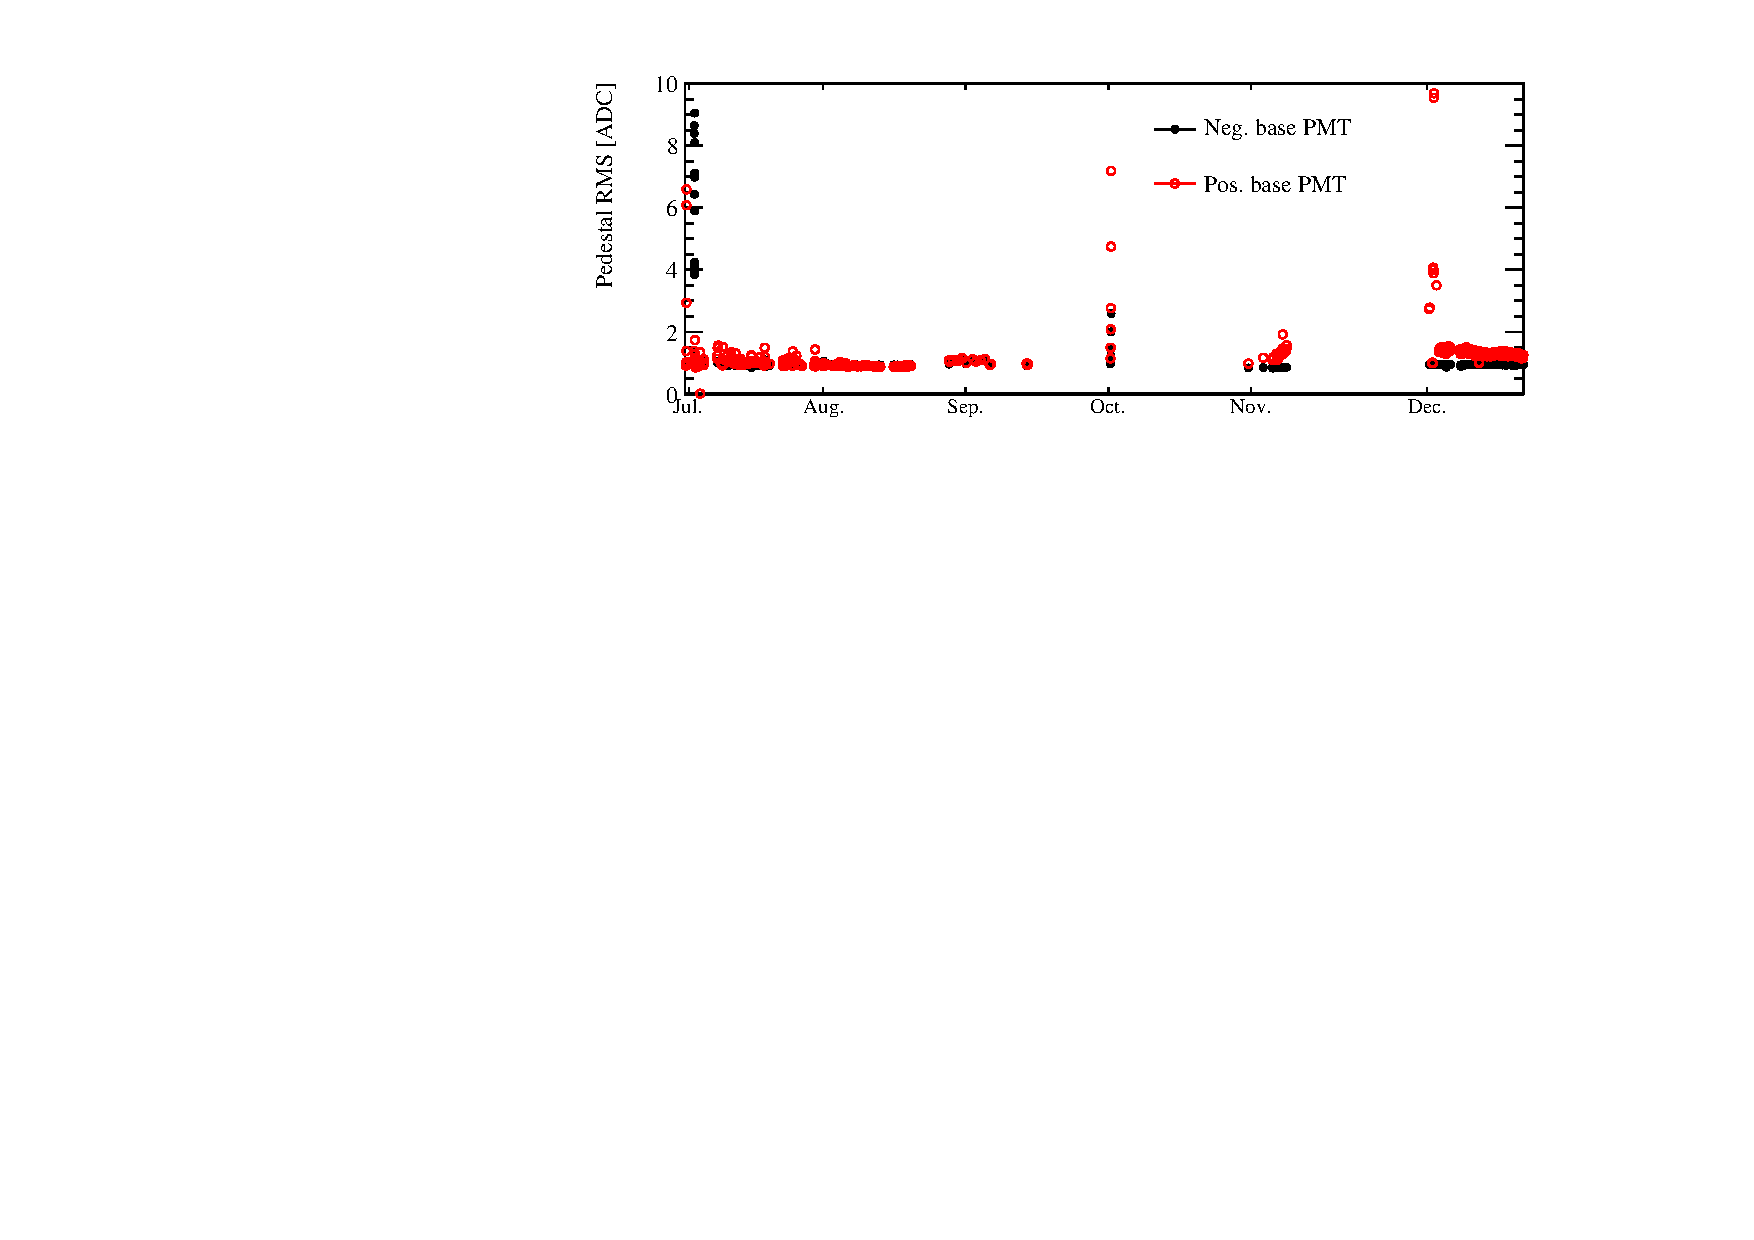
\includegraphics[width=0.9\textwidth]{graphics/dppd_311_pedestal_rms.pdf}
\end{dunefigure}

Figure~\ref{fig:pd-pds-311-LAr-GAr} shows the average waveforms for \dword{pmt} 5 in gas and liquid argon with no drift field. These waveforms are fitted with a gaussian to describe the response function convoluted with a sum of three exponentials to describe the fast, slow, and intermediate components. 
The extracted values agree with the literature, although the lifetime of the fast component has been fixed at \SI{6}{ns} in the fitting procedure.

\begin{dunefigure}[GAr and LAr scintillation profile in WA105]{fig:pd-pds-311-LAr-GAr}{Scintillation time profile in the absence of drift field recorded in GAr (left) and LAr (right) in black. In red, the fit performed with a sum of 3 exponentials (describing the fast, intermediate, and slow components, all shown as dotted blue lines) convoluted with a gaussian to take into account the response function of the \dword{pmt}. The extracted lifetimes are shown in the figure.}
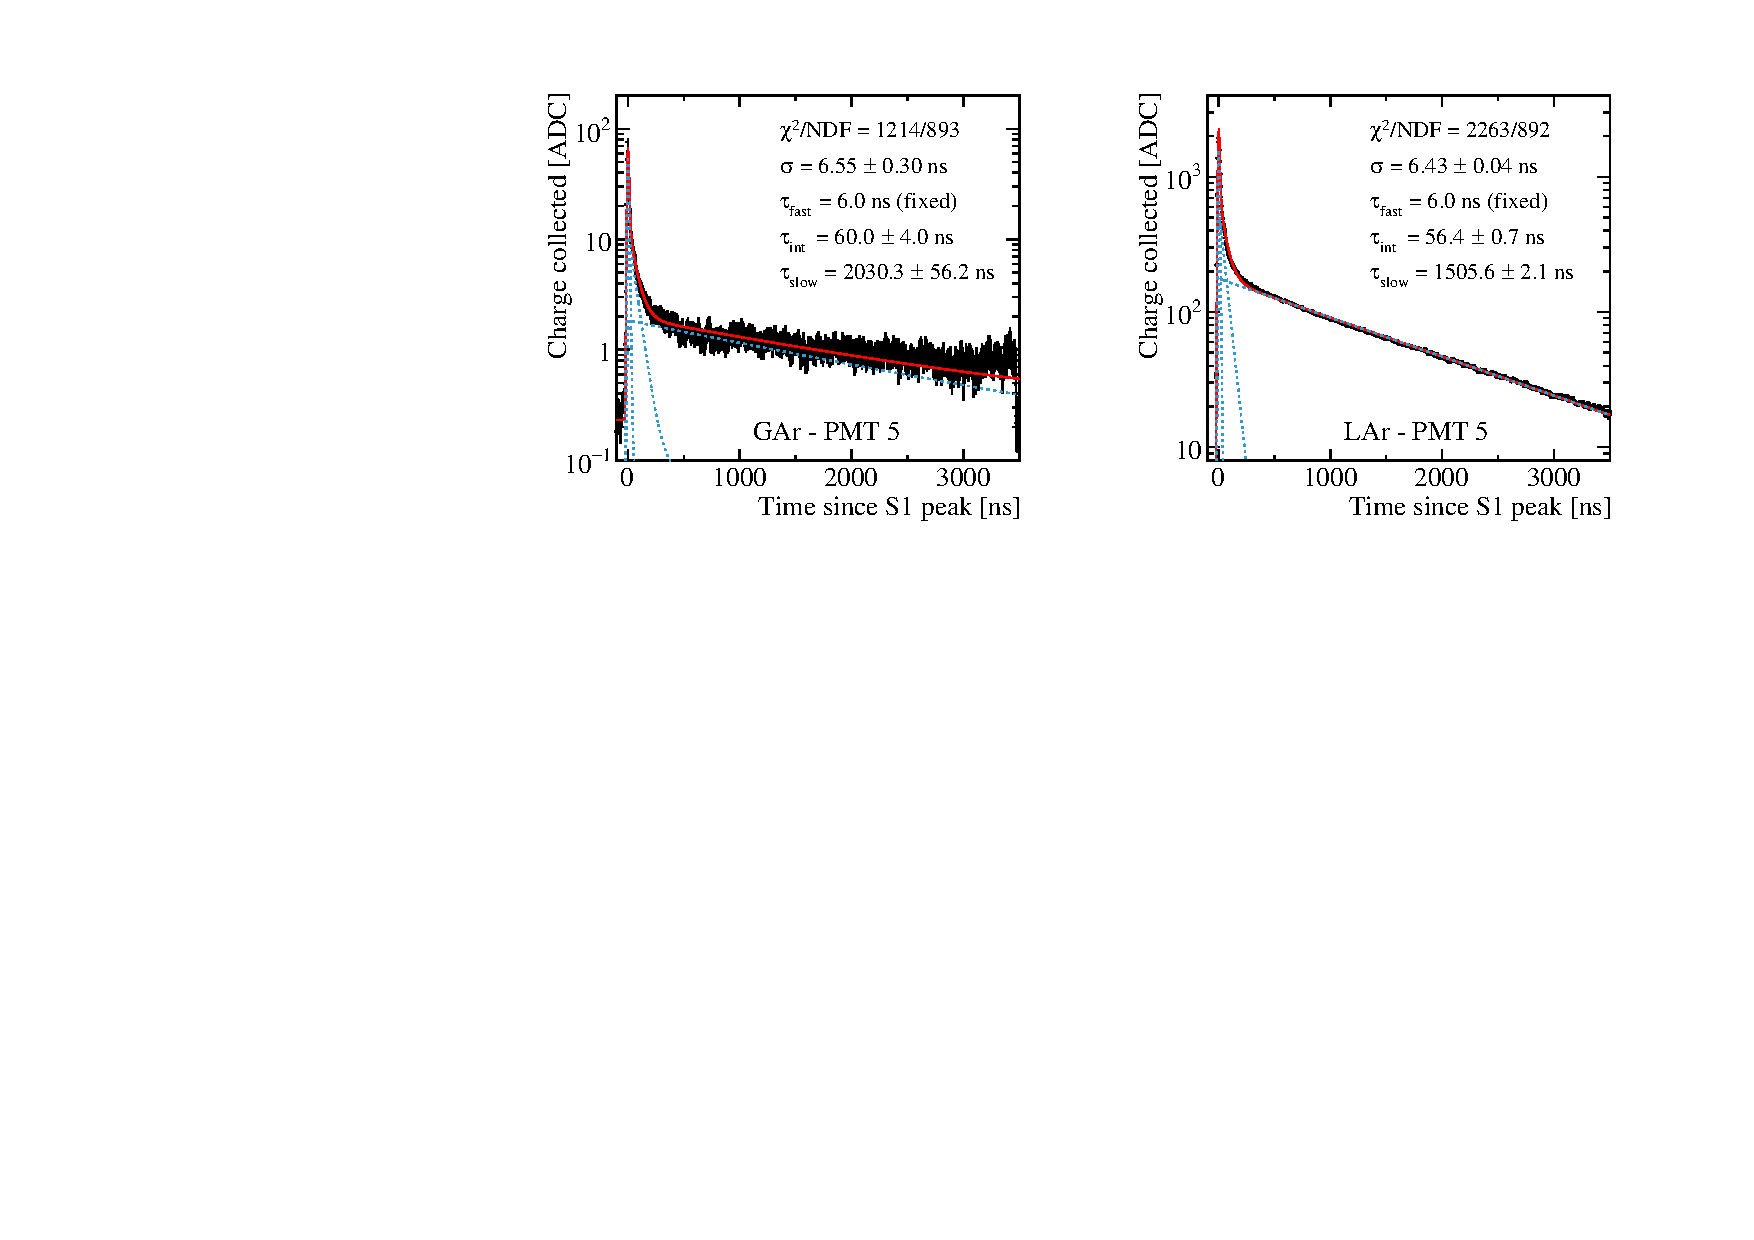
\includegraphics[width=0.85\textwidth]{graphics/dppd_311_lar_gar_fit.pdf}
\end{dunefigure}

Many studies show that $\tau_{slow}$, the slow component (Section~\ref{sec:dp-pds-overview_scintillation}) is very sensitive to the amount of impurities in the liquid.
To monitor the purity of the liquid argon as a function of time, the same fit has been performed on several runs under similar conditions. 
Figure~\ref{fig:pd-pds-311-purity} presents the evolution of $\tau_{slow}$ for \SI{15}{days} of operation.
The results exhibit a very stable amount of impurities, which agrees with the stability of the electron lifetime measured using the charge collection.

\begin{dunefigure}[Evolution of $\tau_{slow}$ as a function of time in WA105]{fig:pd-pds-311-purity}{Evolution of $\tau_{slow}$ over \num{15} days of operation of the \dword{wa105}. The points are the averages over the values extracted from the fits to the waveforms of the \num{3} negative base \dwords{pmt} for runs taken with no drift field. Preliminary results.}
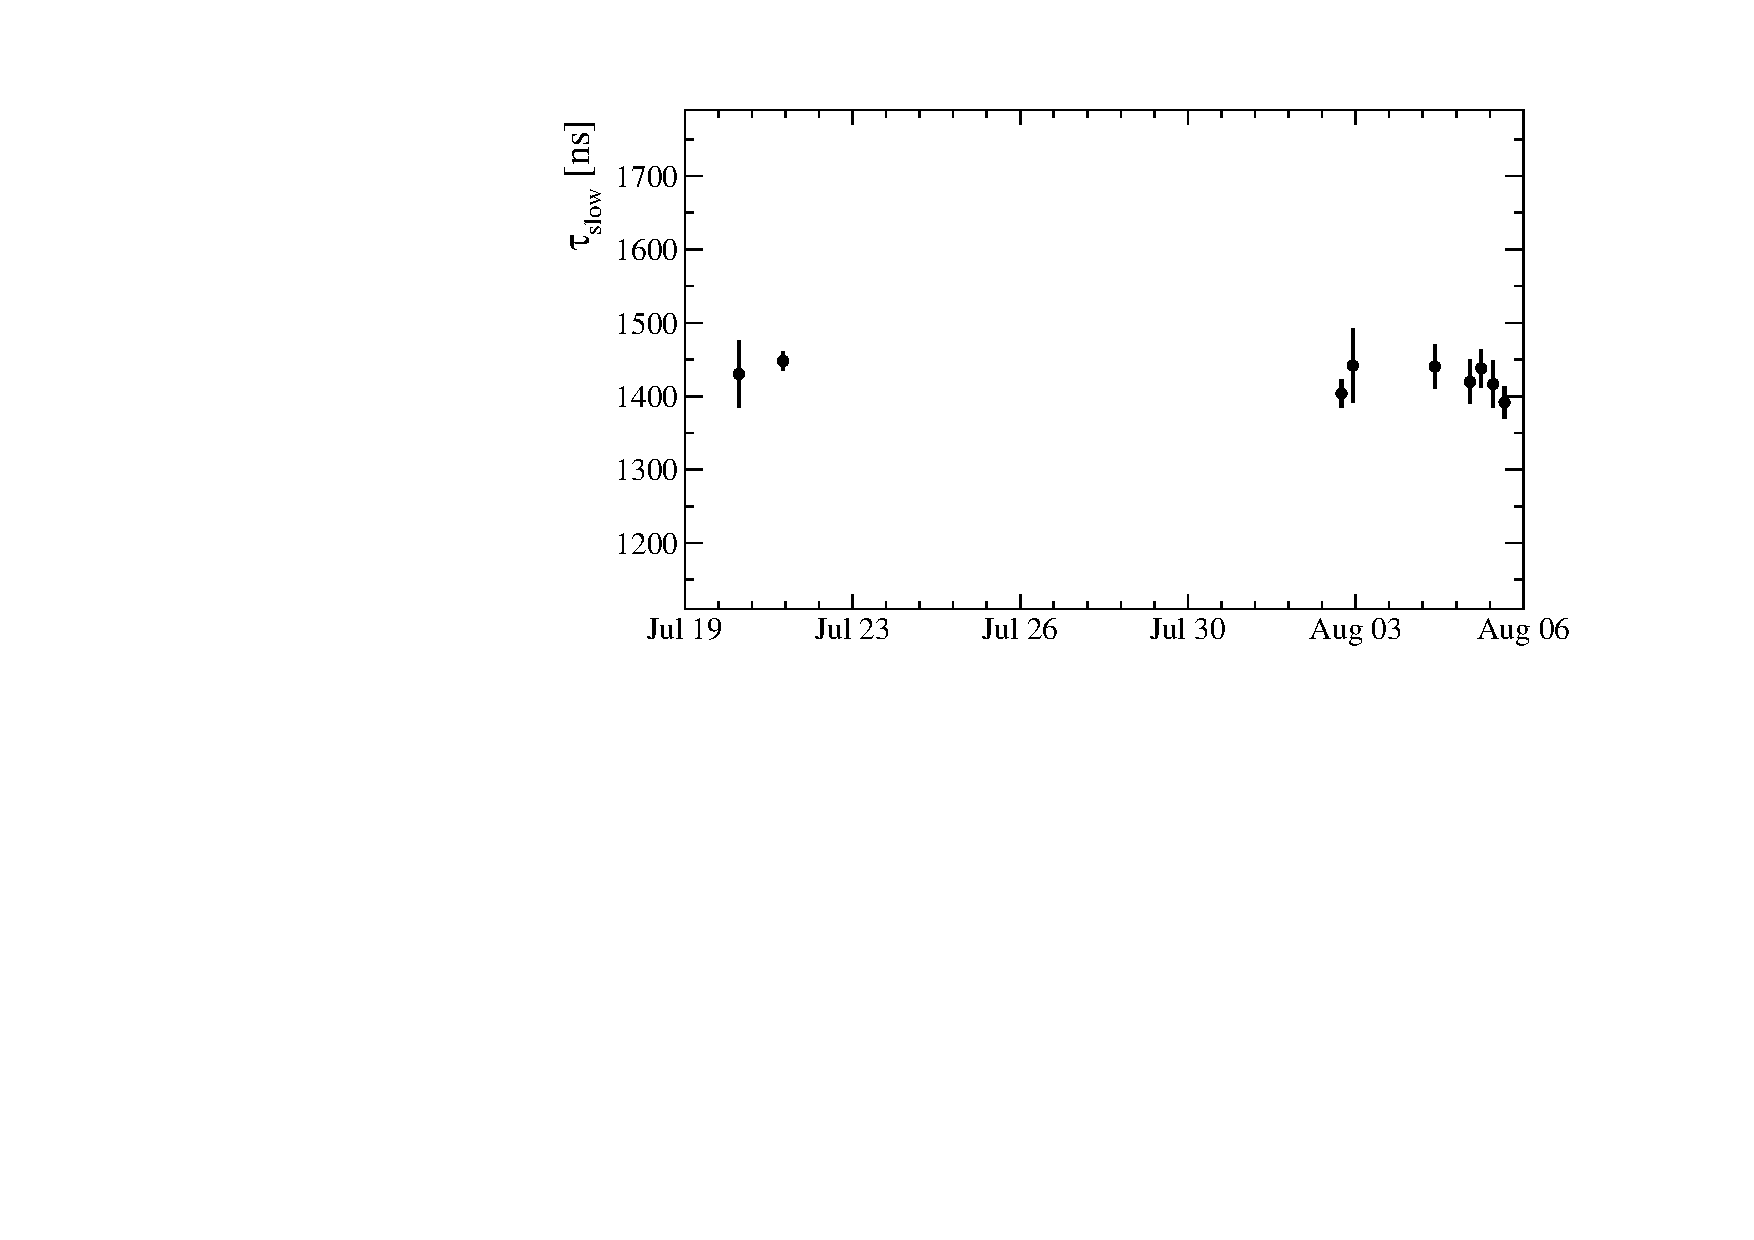
\includegraphics[width=0.7\textwidth]{graphics/dppd_311_purity.pdf}
\end{dunefigure}

The S2 light has also been recorded in dedicated runs using a \SI{1}{ms} recording time window.
Figure~\ref{fig:pd-pds-311-S2} shows the average waveforms from runs with a drift field of \SI{0.5}{kV/cm} and an extraction field of \SI{2}{kV/cm} (\SI{3}{kV/cm}) in liquid (gas). In the figure, one run has no amplification field, the others have the \dwords{lem} polarized to provide an amplification field of \SI{25.5}{kV/cm}. 
The effect of the \dwords{lem} on the amount of S2 light generated is clear. 
The S2 light extends for about \SI{600}{$\mu$s} after emission of the prompt signal, agreeing with the electron drift time over \SI{1}{m} in such drift field.

\begin{dunefigure}[S2 light at different amplification field in WA105]{fig:pd-pds-311-S2}{Average waveforms of negative based \dwords{pmt} in a \SI{1}{ms} window. Both runs were taken with a drift field of \SI{0.5}{kV/cm} and an extraction field of \SI{3}{kV/cm} in gas. The S2 light extends for about \SI{600}{$\mu$s}, as expected.}
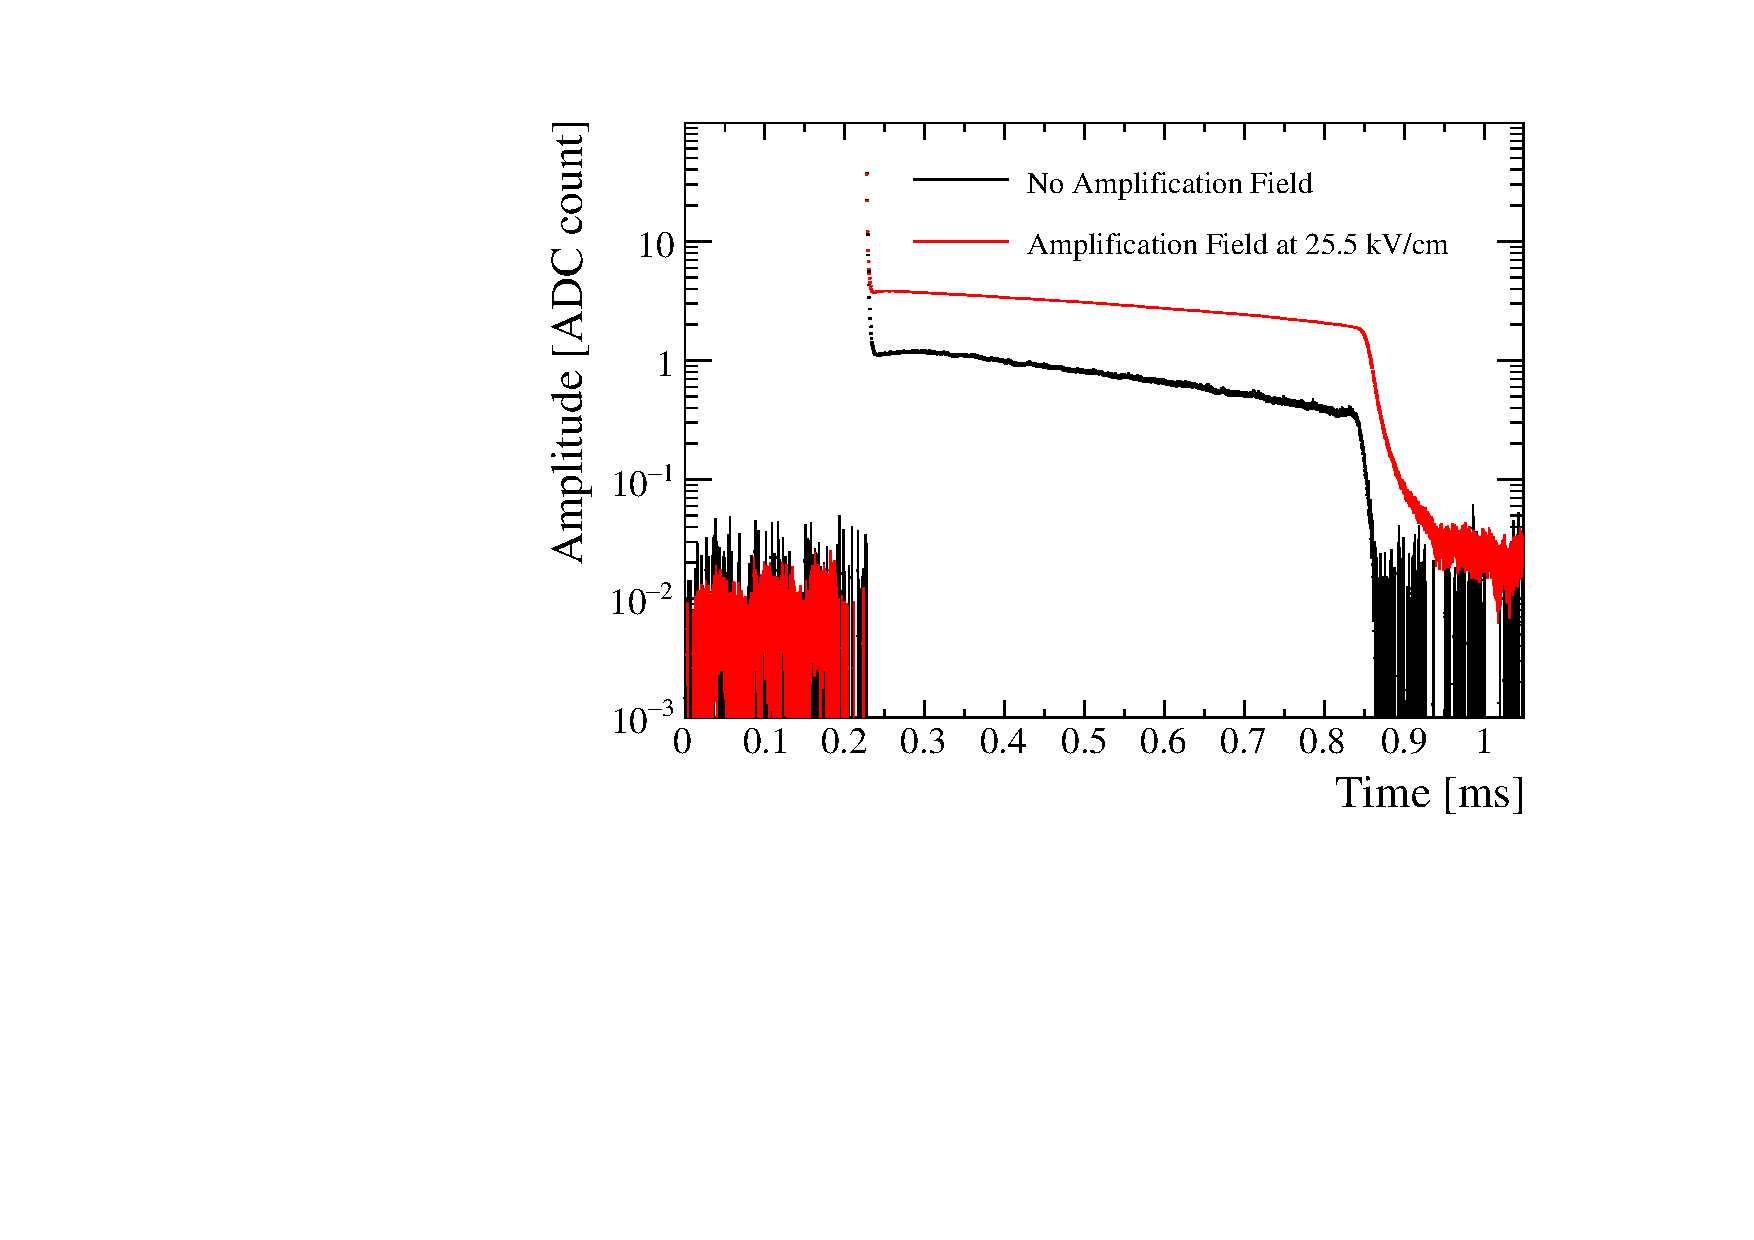
\includegraphics[width=0.7\textwidth]{graphics/dppd_311_S2_extraction.pdf}
\end{dunefigure}
Using data taken at null field in \dword{crt} triggering mode, muon-like tracks are selected. Further, the tracks must cross the active volume for distances longer than \SI{3.1}{\m}. 
The S1 charge collected by each \dword{pmt} is calculated by integrating the \dword{adc} values in a \SI{1}{\us} window starting from the S1 peak; this charge value is then converted into the number of detected \dwords{pe} using the calibrated \dword{pmt} gains in Table~\ref{tab:dp-pds-311conf}.

In the simulation, \SI{4}{\GeV} muons are generated from one \dword{crt} panel to the other with data-driven kinematics. The number of PEs collected by each \dword{pmt} is generated according to the light maps. To suppress spurious triggers, data analysis uses a selection of the minimum amount of light recorded by all \dwords{pmt}; this does not apply to \dword{mc}. Moreover, the \dword{pmt} signal must not saturate the readout only for data analysis, but not \dword{mc}. Figure~\ref{fig:dp-pds-311charge} compares the number of PEs collected in data analysis and in \dword{mc}. The data and \dword{mc} agree well with one another. 

In the \dword{wa105}, the \dword{pmt} gain was adjusted so S1 and S2 light could be seen and thus increase the trigger rate while minimizing the \dword{pmt} \dword{adc} saturation. 
In \dune \dual, the situation will be different as the volume is much larger and part of the triggering modes will be independent from the \dwords{pmt}. 
Hence the \dword{pmt} gain will be adjusted accordingly and the events saturating the ADC should not be as problematic as it could be in \dword{wa105}.
%\fixme{Give more details about why \dword{pmt} saturation in \dword{wa105}, and why this is not worrisome in \dpmod?}

\begin{dunefigure}[Charge collected in WA105 vs MC]{fig:dp-pds-311charge}{ Charge collected by the \dwords{pmt} in a \SI{1}{\us} window containing the S1 peak for muon-like tracks triggered by the \dword{crt} panels. The data is shown in black and the simulation in red. The distributions are normalized to unity for clarity. Preliminary results.}
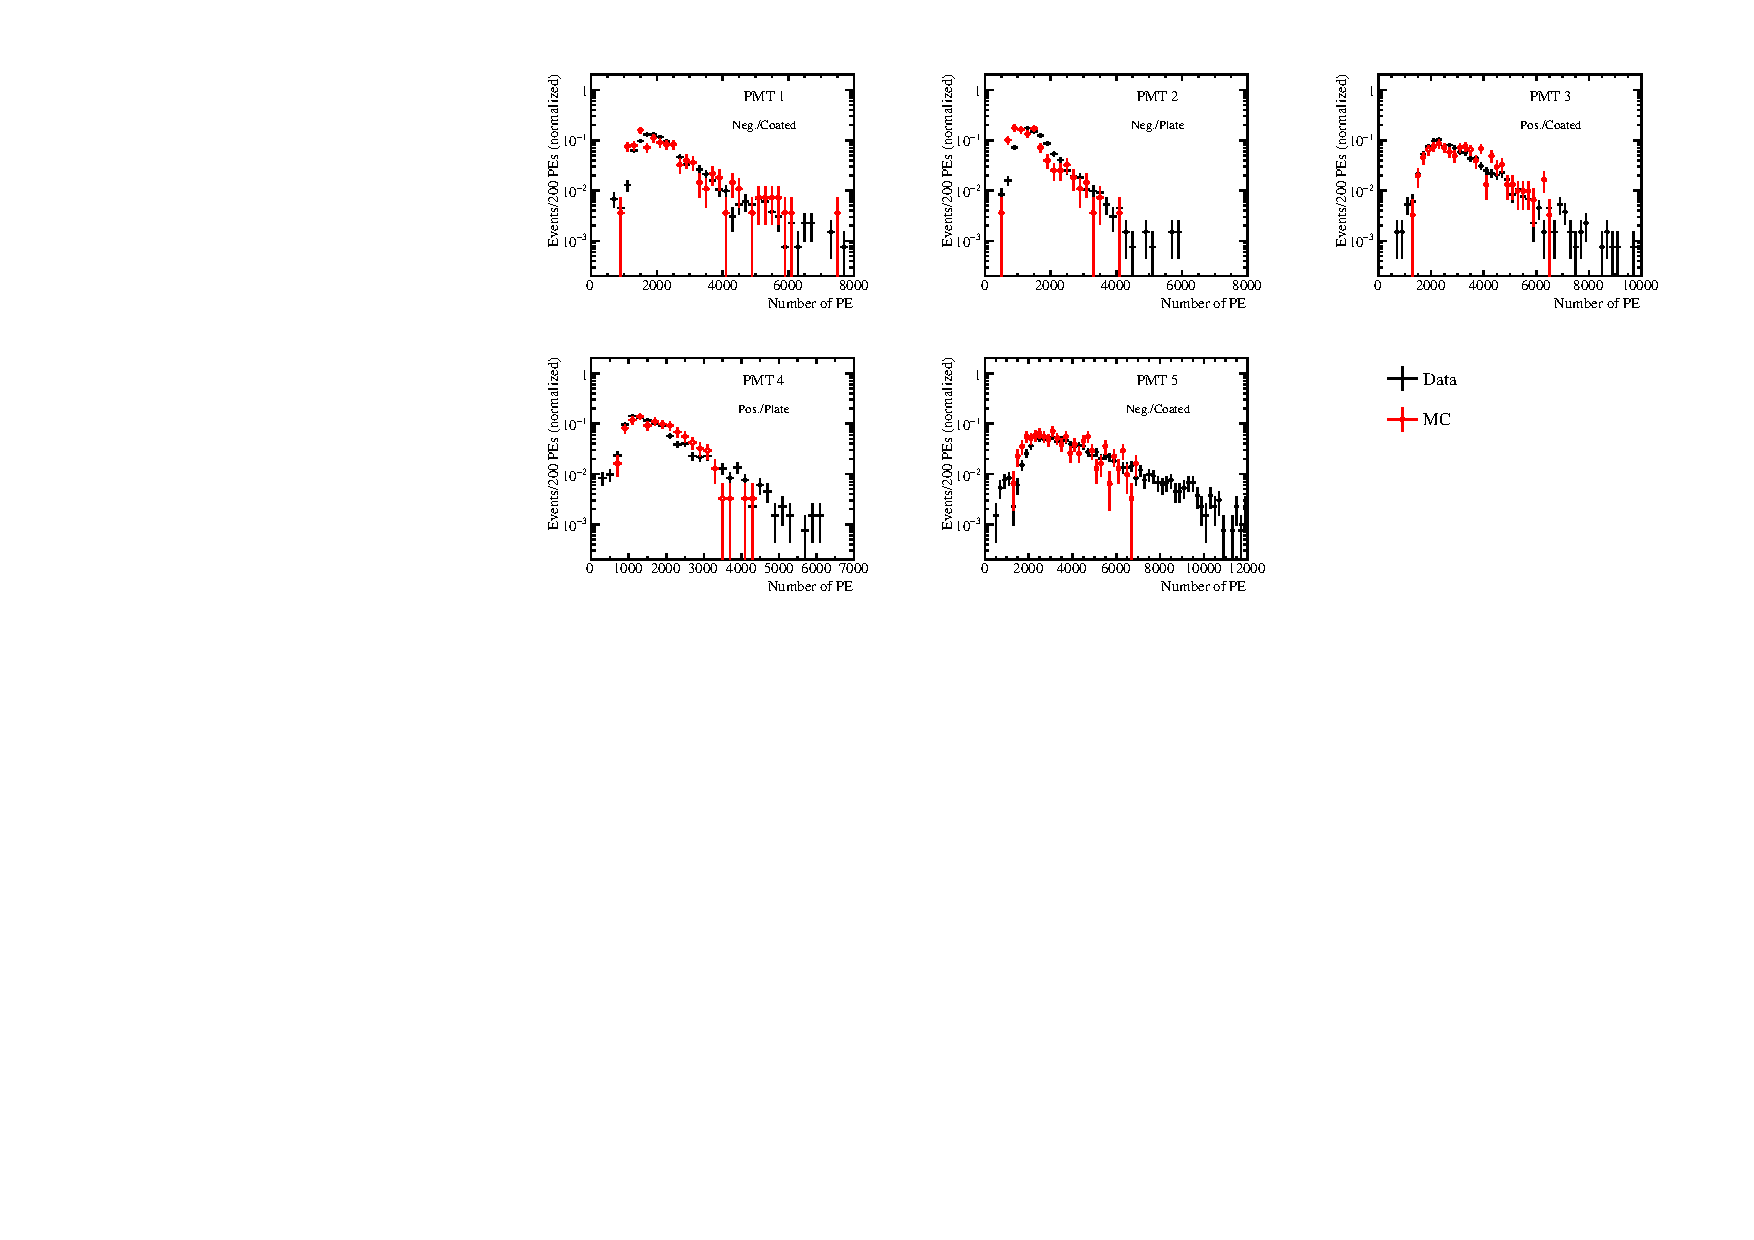
\includegraphics[width=0.95\textwidth]{graphics/dppd_311_charge_mc_v2.pdf}
\end{dunefigure}

\begin{dunefigure}[Charge Collected vs track-PMT shortest distance]{fig:dp-pds-311profile}{Profile histograms of charge collected as a function of the track-PMT shortest distance. The data is in black, the simulation in red. Preliminary results.}
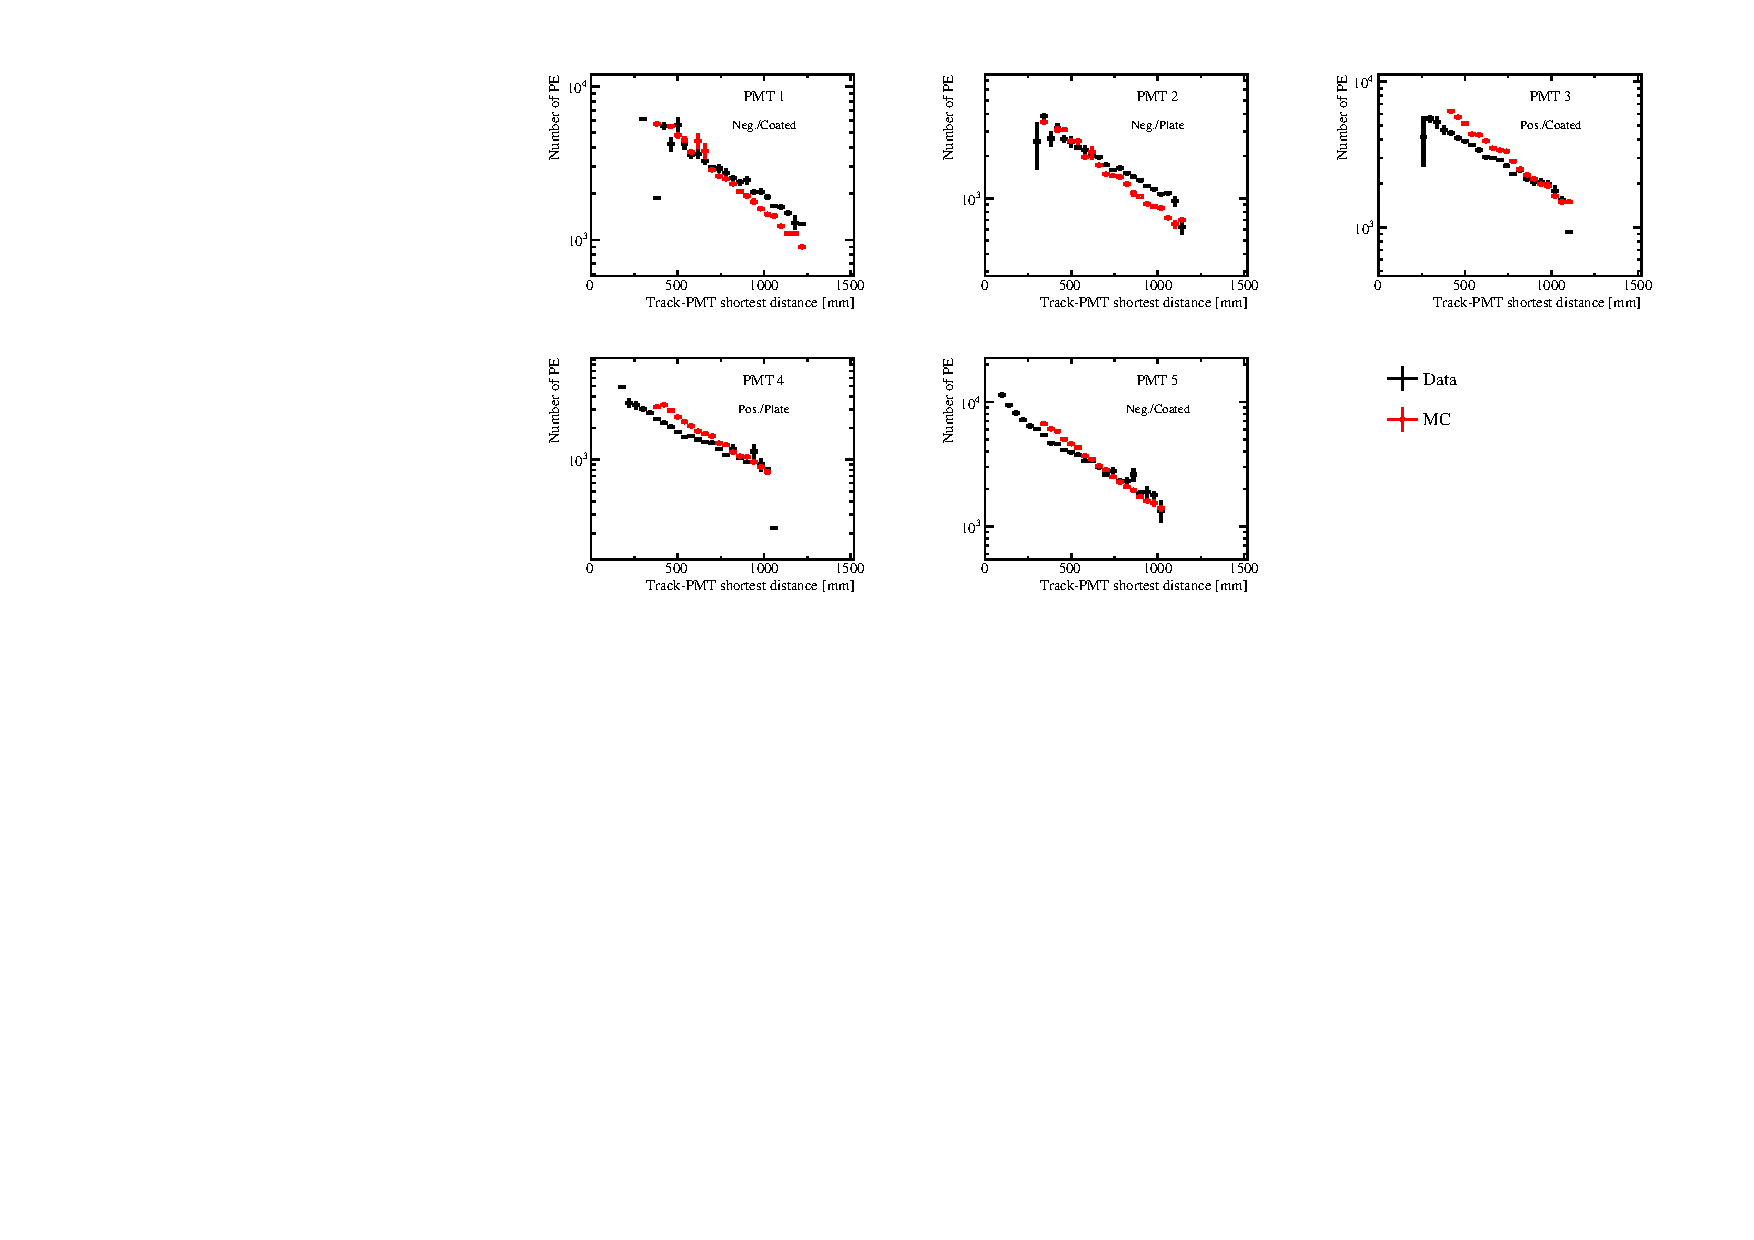
\includegraphics[width=0.95\textwidth]{graphics/dppd_311_charge_dist_mc.pdf}
\end{dunefigure}

%\fixme{This is rather distance vs charge. Is it possible to swap the x and y axis and reproduce the plots?}

The \dwords{pe} collected per \dword{pmt} depends strongly on the shortest track-\dword{pmt} distance. Many factors can affect how much charge is collected, primarily, the scattering length, also known as the Rayleigh scattering length. This quantity is still subject to debate among the \dword{lar} community because its measurement is fairly complicated. Current estimates of the scattering length range from \SI{20}{\cm} to \SI{1}{\m}.
In the \dword{wa105} simulation, the scattering length was set to L$_{ray}$ = \SI{55}{\cm}.
Figure~\ref{fig:dp-pds-311profile} shows the charge collected as a function of the shortest track-\dword{pmt} distance in the form of profile histograms. The overall trend is very similar for data and \dword{mc}, also across all the \dwords{pmt}. However, the profile histogram slopes indicate that the assumed scattering length in \dword{mc} could be better tuned to reproduce the data, e.g., toward larger values of the Rayleigh scattering length.

%%%%%%%%%%%%%%%%%%%%%%%%%%%%%%%%%%%%%%%%%%%%%%%%%%%%%%%%%%%%%%%%%%%%

\subsection{Installation of the \dword{pddp} Photon Detector System}

At the time of writing, no scintillation light data from \dword{pddp} are yet available. Nevertheless, important lessons from \dword{pddp} have already been learned, thanks to the recent installation of its photon detector system. They are summarized below. Figure~\ref{fig:dppd_pmt_installation} shows the placement of the \num{36} \dwords{pmt} in \dword{pddp} on the cryostat floor, performed in February 2019.

\begin{dunefigure}[Installation of the ProtoDUNE-DP PDS]{fig:dppd_pmt_installation}{Installation of the \dword{pddp} photon detector system.}
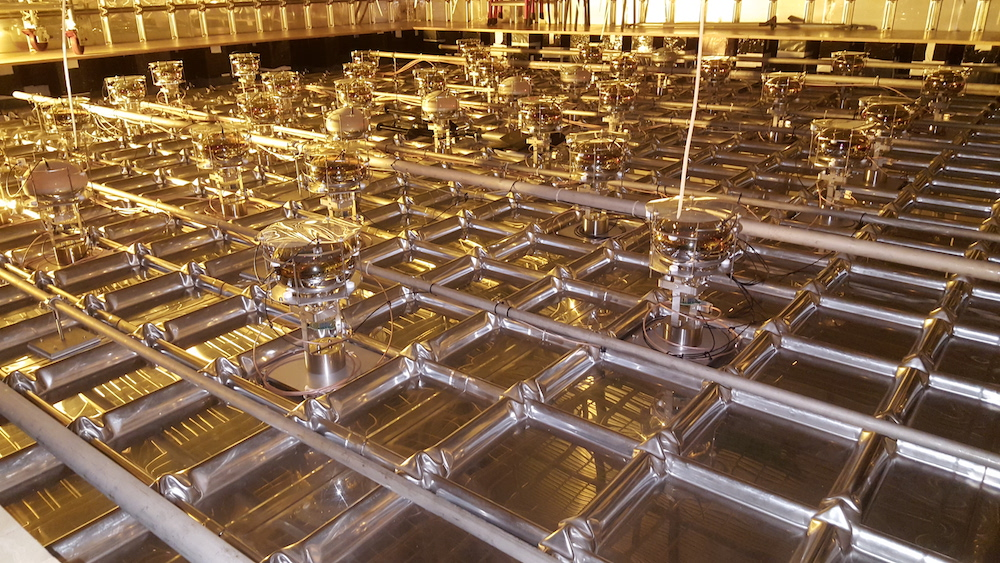
\includegraphics[width=0.8\textwidth]{graphics/dppd_pmt_installation.jpg}
\end{dunefigure}

One of the most critical points of the installation is the order of the tasks. Since the installation activities lasted several days in the \dword{pddp} case, and will last several months for an \dword{fd} module, and given that other persons have to work near the \dword{pds} components, the risk of damage has to be considered. The fragility of the components determines the installation order. The \dword{pmt} supporting bases and the signal-HV \dword{pmt} cables must be be installed first, then the \dwords{pmt} can be mounted on their holders and connected to the cables, and finally the calibration fiber system has to be installed. The need of protecting the components has to be evaluated if there are subsequent activities around them. For example, Figure~\ref{fig:dppd_pmt_installation} shows how temporary protective plates were placed in front of the \dword{pddp} \dword{pmt} photo-cathodes, and the \dword{pmt} units were enclosed in temporary plastic bags. 

The conceptual division of the \dword{fd} \dword{pds} into several sectors is crucial. In \dword{pddp}, the \num{36} \dwords{pmt} were divided into six groups of \num{6} \dwords{pmt} each. This arrangement simplified the installation of the calibration fibers considering that each fiber bundle has \num{7} fibers, including one spare fiber per bundle. 

Concerning organizational matters, \dword{pddp} experience shows that several documents should be prepared prior to installation, including a detailed description of all the tasks to be performed, a time estimation for all of them, and a list of the necessary items. In addition, the required status of the detector before each installation stage should be indicated. This information must be as detailed as possible. The benefits of a detailed planning are:

\begin{itemize}
\item All the persons participating in the \dword{pds} installation know their roles.
\item The required material is foreseen and available when needed.
\item The interaction with other installation crews is planned.
\item The expected time for the installation is known in advance and extra time for unexpected events can be added.
\item It is possible to communicate beforehand all the requests to the coordinator of the installation.
\item The overlapping of activities and the waiting times are minimized. 
\end{itemize}
